\documentclass[twoside]{book}

% Packages required by doxygen
\usepackage{fixltx2e}
\usepackage{calc}
\usepackage{doxygen}
\usepackage[export]{adjustbox} % also loads graphicx
\usepackage{graphicx}
\usepackage[utf8]{inputenc}
\usepackage{makeidx}
\usepackage{multicol}
\usepackage{multirow}
\PassOptionsToPackage{warn}{textcomp}
\usepackage{textcomp}
\usepackage[nointegrals]{wasysym}
\usepackage[table]{xcolor}

% Font selection
\usepackage[T1]{fontenc}
\usepackage[scaled=.90]{helvet}
\usepackage{courier}
\usepackage{amssymb}
\usepackage{sectsty}
\renewcommand{\familydefault}{\sfdefault}
\allsectionsfont{%
  \fontseries{bc}\selectfont%
  \color{darkgray}%
}
\renewcommand{\DoxyLabelFont}{%
  \fontseries{bc}\selectfont%
  \color{darkgray}%
}
\newcommand{\+}{\discretionary{\mbox{\scriptsize$\hookleftarrow$}}{}{}}

% Page & text layout
\usepackage{geometry}
\geometry{%
  a4paper,%
  top=2.5cm,%
  bottom=2.5cm,%
  left=2.5cm,%
  right=2.5cm%
}
\tolerance=750
\hfuzz=15pt
\hbadness=750
\setlength{\emergencystretch}{15pt}
\setlength{\parindent}{0cm}
\setlength{\parskip}{3ex plus 2ex minus 2ex}
\makeatletter
\renewcommand{\paragraph}{%
  \@startsection{paragraph}{4}{0ex}{-1.0ex}{1.0ex}{%
    \normalfont\normalsize\bfseries\SS@parafont%
  }%
}
\renewcommand{\subparagraph}{%
  \@startsection{subparagraph}{5}{0ex}{-1.0ex}{1.0ex}{%
    \normalfont\normalsize\bfseries\SS@subparafont%
  }%
}
\makeatother

% Headers & footers
\usepackage{fancyhdr}
\pagestyle{fancyplain}
\fancyhead[LE]{\fancyplain{}{\bfseries\thepage}}
\fancyhead[CE]{\fancyplain{}{}}
\fancyhead[RE]{\fancyplain{}{\bfseries\leftmark}}
\fancyhead[LO]{\fancyplain{}{\bfseries\rightmark}}
\fancyhead[CO]{\fancyplain{}{}}
\fancyhead[RO]{\fancyplain{}{\bfseries\thepage}}
\fancyfoot[LE]{\fancyplain{}{}}
\fancyfoot[CE]{\fancyplain{}{}}
\fancyfoot[RE]{\fancyplain{}{\bfseries\scriptsize Generated by Doxygen }}
\fancyfoot[LO]{\fancyplain{}{\bfseries\scriptsize Generated by Doxygen }}
\fancyfoot[CO]{\fancyplain{}{}}
\fancyfoot[RO]{\fancyplain{}{}}
\renewcommand{\footrulewidth}{0.4pt}
\renewcommand{\chaptermark}[1]{%
  \markboth{#1}{}%
}
\renewcommand{\sectionmark}[1]{%
  \markright{\thesection\ #1}%
}

% Indices & bibliography
\usepackage{natbib}
\usepackage[titles]{tocloft}
\setcounter{tocdepth}{3}
\setcounter{secnumdepth}{5}
\makeindex

% Hyperlinks (required, but should be loaded last)
\usepackage{ifpdf}
\ifpdf
  \usepackage[pdftex,pagebackref=true]{hyperref}
\else
  \usepackage[ps2pdf,pagebackref=true]{hyperref}
\fi
\hypersetup{%
  colorlinks=true,%
  linkcolor=blue,%
  citecolor=blue,%
  unicode%
}

% Custom commands
\newcommand{\clearemptydoublepage}{%
  \newpage{\pagestyle{empty}\cleardoublepage}%
}

\usepackage{caption}
\captionsetup{labelsep=space,justification=centering,font={bf},singlelinecheck=off,skip=4pt,position=top}

%===== C O N T E N T S =====

\begin{document}

% Titlepage & ToC
\hypersetup{pageanchor=false,
             bookmarksnumbered=true,
             pdfencoding=unicode
            }
\pagenumbering{alph}
\begin{titlepage}
\vspace*{7cm}
\begin{center}%
{\Large Elevator }\\
\vspace*{1cm}
{\large Generated by Doxygen 1.8.13}\\
\end{center}
\end{titlepage}
\clearemptydoublepage
\pagenumbering{roman}
\tableofcontents
\clearemptydoublepage
\pagenumbering{arabic}
\hypersetup{pageanchor=true}

%--- Begin generated contents ---
\chapter{Data Structure Index}
\section{Data Structures}
Here are the data structures with brief descriptions\+:\begin{DoxyCompactList}
\item\contentsline{section}{\hyperlink{structDirection}{Direction} \\*Define a struct to keep track of current and previous direction }{\pageref{structDirection}}{}
\item\contentsline{section}{\hyperlink{structFloor}{Floor} \\*Define a struct to keep track of current and previous floors }{\pageref{structFloor}}{}
\end{DoxyCompactList}

\chapter{File Index}
\section{File List}
Here is a list of all documented files with brief descriptions\+:\begin{DoxyCompactList}
\item\contentsline{section}{source/\hyperlink{elevatorLogic_8c}{elevator\+Logic.\+c} \\*Implementation file elevator logic }{\pageref{elevatorLogic_8c}}{}
\item\contentsline{section}{source/\hyperlink{elevatorLogic_8h}{elevator\+Logic.\+h} \\*Functions that decide what the elevetaor will do at a given time and state }{\pageref{elevatorLogic_8h}}{}
\item\contentsline{section}{source/\hyperlink{hardware_8h}{hardware.\+h} \\*Driver for the elevator hardware }{\pageref{hardware_8h}}{}
\item\contentsline{section}{source/\hyperlink{helpFunctions_8c}{help\+Functions.\+c} \\*Implementation file for help\+Functions }{\pageref{helpFunctions_8c}}{}
\item\contentsline{section}{source/\hyperlink{helpFunctions_8h}{help\+Functions.\+h} \\*Small functions with intuitive behavior that are used in {\ttfamily \hyperlink{elevatorLogic_8c}{elevator\+Logic.\+c}} }{\pageref{helpFunctions_8h}}{}
\item\contentsline{section}{source/\hyperlink{main_8c}{main.\+c} \\*The main file of the application }{\pageref{main_8c}}{}
\item\contentsline{section}{source/\hyperlink{timer_8c}{timer.\+c} \\*Implementation file for timer }{\pageref{timer_8c}}{}
\item\contentsline{section}{source/\hyperlink{timer_8h}{timer.\+h} \\*Functions to keep track of how long certain operations has last }{\pageref{timer_8h}}{}
\item\contentsline{section}{source/\hyperlink{variables_8h}{variables.\+h} \\*Define global variables }{\pageref{variables_8h}}{}
\end{DoxyCompactList}

\chapter{Data Structure Documentation}
\hypertarget{structDirection}{}\section{Direction Struct Reference}
\label{structDirection}\index{Direction@{Direction}}


Define a struct to keep track of current and previous direction.  




{\ttfamily \#include $<$variables.\+h$>$}

\subsection*{Data Fields}
\begin{DoxyCompactItemize}
\item 
\mbox{\Hypertarget{structDirection_a9a25b1f4fa501943844ed3163d8d206f}\label{structDirection_a9a25b1f4fa501943844ed3163d8d206f}} 
\hyperlink{hardware_8h_a2167c399a24df296afc432bcb88228af}{Hardware\+Movement} {\bfseries current}
\item 
\mbox{\Hypertarget{structDirection_a6615cfe7b8c667d52f863664e15059a3}\label{structDirection_a6615cfe7b8c667d52f863664e15059a3}} 
\hyperlink{hardware_8h_a2167c399a24df296afc432bcb88228af}{Hardware\+Movement} {\bfseries last}
\end{DoxyCompactItemize}


\subsection{Detailed Description}
Define a struct to keep track of current and previous direction. 


\begin{DoxyParams}{Parameters}
{\em current} & Holds the current direction. \\
\hline
{\em last} & Holds the last direction the elevator had when it was moving. \\
\hline
\end{DoxyParams}


Definition at line 29 of file variables.\+h.



The documentation for this struct was generated from the following file\+:\begin{DoxyCompactItemize}
\item 
source/\hyperlink{variables_8h}{variables.\+h}\end{DoxyCompactItemize}

\hypertarget{structFloor}{}\section{Floor Struct Reference}
\label{structFloor}\index{Floor@{Floor}}


Define a struct to keep track of current and previous floors.  




{\ttfamily \#include $<$variables.\+h$>$}

\subsection*{Data Fields}
\begin{DoxyCompactItemize}
\item 
\mbox{\Hypertarget{structFloor_a5a00f2754bbc65702117716a5e7d87d4}\label{structFloor_a5a00f2754bbc65702117716a5e7d87d4}} 
int {\bfseries current}
\item 
\mbox{\Hypertarget{structFloor_ac90720369c3ed4f179214eede559224d}\label{structFloor_ac90720369c3ed4f179214eede559224d}} 
int {\bfseries last}
\end{DoxyCompactItemize}


\subsection{Detailed Description}
Define a struct to keep track of current and previous floors. 


\begin{DoxyParams}{Parameters}
{\em current} & Holds the current floor. -\/1 if moving. \\
\hline
{\em last} & Holds the last floor. \\
\hline
\end{DoxyParams}


Definition at line 18 of file variables.\+h.



The documentation for this struct was generated from the following file\+:\begin{DoxyCompactItemize}
\item 
source/\hyperlink{variables_8h}{variables.\+h}\end{DoxyCompactItemize}

\chapter{File Documentation}
\hypertarget{elevatorLogic_8c}{}\section{source/elevator\+Logic.c File Reference}
\label{elevatorLogic_8c}\index{source/elevator\+Logic.\+c@{source/elevator\+Logic.\+c}}


Implementation file elevator logic.  


{\ttfamily \#include \char`\"{}elevator\+Logic.\+h\char`\"{}}\newline
Include dependency graph for elevator\+Logic.\+c\+:
\nopagebreak
\begin{figure}[H]
\begin{center}
\leavevmode
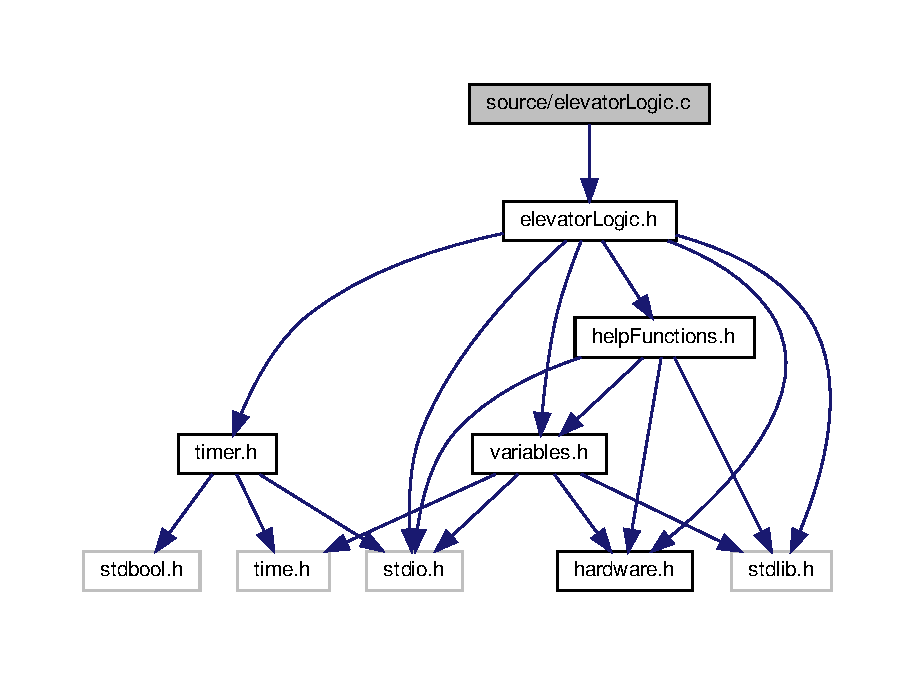
\includegraphics[width=350pt]{elevatorLogic_8c__incl}
\end{center}
\end{figure}
\subsection*{Functions}
\begin{DoxyCompactItemize}
\item 
\mbox{\Hypertarget{elevatorLogic_8c_a5b7e520dd3634bc511e199023a2a4ad5}\label{elevatorLogic_8c_a5b7e520dd3634bc511e199023a2a4ad5}} 
void \hyperlink{elevatorLogic_8c_a5b7e520dd3634bc511e199023a2a4ad5}{initialize\+Elevator} ()
\begin{DoxyCompactList}\small\item\em Resets lights, and drives down until the elevator reaches a floor sensor. Saves this floor as {\ttfamily F\+L\+O\+O\+R.\+current} and {\ttfamily F\+L\+O\+O\+R.\+last}. \end{DoxyCompactList}\item 
int \hyperlink{elevatorLogic_8c_acb58ac12f71a53ca9d454ea0bef0859c}{check\+If\+Stop} ()
\begin{DoxyCompactList}\small\item\em When the elevator is moving and reaches a floor, the floor indicator lights up, {\ttfamily F\+L\+O\+O\+R.\+last} is set, and it decides whether or not to stop at this floor. \end{DoxyCompactList}\item 
\mbox{\Hypertarget{elevatorLogic_8c_a0348ac8c5f50ff4dd510de9905f5d858}\label{elevatorLogic_8c_a0348ac8c5f50ff4dd510de9905f5d858}} 
void \hyperlink{elevatorLogic_8c_a0348ac8c5f50ff4dd510de9905f5d858}{arrive\+Floor} ()
\begin{DoxyCompactList}\small\item\em As long as the {\ttfamily has\+Just\+Left} flag is not set, this function stops the elevator, starts the timer, open the door, and deletes the order to the current floor. \end{DoxyCompactList}\item 
\mbox{\Hypertarget{elevatorLogic_8c_a8259fdde833753b6f23004be29dbb56c}\label{elevatorLogic_8c_a8259fdde833753b6f23004be29dbb56c}} 
void \hyperlink{elevatorLogic_8c_a8259fdde833753b6f23004be29dbb56c}{leave\+Floor} ()
\begin{DoxyCompactList}\small\item\em When the timer reaches 3 seconds and the elevator is not moving, the door is closed and new orders are looked for using {\ttfamily \hyperlink{elevatorLogic_8h_a949e2c521323a4e0d2c37c79c275def5}{update\+Direction()}}. \end{DoxyCompactList}\item 
\mbox{\Hypertarget{elevatorLogic_8c_a2c615610a51b585d757c6fd48c0ea577}\label{elevatorLogic_8c_a2c615610a51b585d757c6fd48c0ea577}} 
void {\bfseries update\+Direction} (int any\+Orders\+Above, int any\+Orders\+Below)
\item 
\mbox{\Hypertarget{elevatorLogic_8c_a98ff2b0015e3c6361fdeec413d689f30}\label{elevatorLogic_8c_a98ff2b0015e3c6361fdeec413d689f30}} 
void \hyperlink{elevatorLogic_8c_a98ff2b0015e3c6361fdeec413d689f30}{set\+Orders\+And\+Order\+Lights} ()
\begin{DoxyCompactList}\small\item\em Polls all order buttons, and sets {\ttfamily M\+A\+S\+T\+E\+R\+\_\+\+M\+A\+T\+R\+IX} and the corresponding light if any buttons are pushed. \end{DoxyCompactList}\item 
\mbox{\Hypertarget{elevatorLogic_8c_a19e50b36bc41e271ad3d4e4ac86bb9c3}\label{elevatorLogic_8c_a19e50b36bc41e271ad3d4e4ac86bb9c3}} 
void \hyperlink{elevatorLogic_8c_a19e50b36bc41e271ad3d4e4ac86bb9c3}{stop\+Function} ()
\begin{DoxyCompactList}\small\item\em Stops the elevator, sets {\ttfamily has\+Stopped} to 1 and flushes all orders. If the elevator is at a floor, the door is opened. Sets the stoplight. \end{DoxyCompactList}\item 
\mbox{\Hypertarget{elevatorLogic_8c_af80114ed5f35a4a3facbf60811b46821}\label{elevatorLogic_8c_af80114ed5f35a4a3facbf60811b46821}} 
void \hyperlink{elevatorLogic_8c_af80114ed5f35a4a3facbf60811b46821}{has\+Stopped\+Function} ()
\begin{DoxyCompactList}\small\item\em If the elevator has stopped between two floors, this function determines these two floors and calls {\ttfamily \hyperlink{elevatorLogic_8h_a949e2c521323a4e0d2c37c79c275def5}{update\+Direction()}} with the result as the two parameters. \end{DoxyCompactList}\item 
\mbox{\Hypertarget{elevatorLogic_8c_a629b2358b6d36a8f0312246b38c962eb}\label{elevatorLogic_8c_a629b2358b6d36a8f0312246b38c962eb}} 
void \hyperlink{elevatorLogic_8c_a629b2358b6d36a8f0312246b38c962eb}{check\+For\+Orders\+On\+Current\+Floor} ()
\begin{DoxyCompactList}\small\item\em If the elevator is ordered at its {\ttfamily F\+L\+O\+O\+R.\+current}, {\ttfamily \hyperlink{elevatorLogic_8h_a0348ac8c5f50ff4dd510de9905f5d858}{arrive\+Floor()}} is called. \end{DoxyCompactList}\item 
int \hyperlink{elevatorLogic_8c_a59e7425ac35298bb95a7c2d224a87d98}{check\+For\+Obstruction} ()
\begin{DoxyCompactList}\small\item\em Determines wheter the obstruction switch should have any effect. \end{DoxyCompactList}\end{DoxyCompactItemize}


\subsection{Detailed Description}
Implementation file elevator logic. 



\subsection{Function Documentation}
\mbox{\Hypertarget{elevatorLogic_8c_a59e7425ac35298bb95a7c2d224a87d98}\label{elevatorLogic_8c_a59e7425ac35298bb95a7c2d224a87d98}} 
\index{elevator\+Logic.\+c@{elevator\+Logic.\+c}!check\+For\+Obstruction@{check\+For\+Obstruction}}
\index{check\+For\+Obstruction@{check\+For\+Obstruction}!elevator\+Logic.\+c@{elevator\+Logic.\+c}}
\subsubsection{\texorpdfstring{check\+For\+Obstruction()}{checkForObstruction()}}
{\footnotesize\ttfamily int check\+For\+Obstruction (\begin{DoxyParamCaption}{ }\end{DoxyParamCaption})}



Determines wheter the obstruction switch should have any effect. 

\begin{DoxyReturn}{Returns}
1 if the obstruction switch should affect the elevator, 0 if not. 
\end{DoxyReturn}


Definition at line 147 of file elevator\+Logic.\+c.

\mbox{\Hypertarget{elevatorLogic_8c_acb58ac12f71a53ca9d454ea0bef0859c}\label{elevatorLogic_8c_acb58ac12f71a53ca9d454ea0bef0859c}} 
\index{elevator\+Logic.\+c@{elevator\+Logic.\+c}!check\+If\+Stop@{check\+If\+Stop}}
\index{check\+If\+Stop@{check\+If\+Stop}!elevator\+Logic.\+c@{elevator\+Logic.\+c}}
\subsubsection{\texorpdfstring{check\+If\+Stop()}{checkIfStop()}}
{\footnotesize\ttfamily int check\+If\+Stop (\begin{DoxyParamCaption}{ }\end{DoxyParamCaption})}



When the elevator is moving and reaches a floor, the floor indicator lights up, {\ttfamily F\+L\+O\+O\+R.\+last} is set, and it decides whether or not to stop at this floor. 

\begin{DoxyReturn}{Returns}
0 if the elevator is to drive past the floor. 1 to stop. 
\end{DoxyReturn}


Definition at line 25 of file elevator\+Logic.\+c.


\hypertarget{elevatorLogic_8h}{}\section{source/elevator\+Logic.h File Reference}
\label{elevatorLogic_8h}\index{source/elevator\+Logic.\+h@{source/elevator\+Logic.\+h}}


Functions that decide what the elevetaor will do at a given time and state.  


{\ttfamily \#include $<$stdio.\+h$>$}\newline
{\ttfamily \#include $<$stdlib.\+h$>$}\newline
{\ttfamily \#include \char`\"{}hardware.\+h\char`\"{}}\newline
{\ttfamily \#include \char`\"{}timer.\+h\char`\"{}}\newline
{\ttfamily \#include \char`\"{}variables.\+h\char`\"{}}\newline
{\ttfamily \#include \char`\"{}help\+Functions.\+h\char`\"{}}\newline
Include dependency graph for elevator\+Logic.\+h\+:
\nopagebreak
\begin{figure}[H]
\begin{center}
\leavevmode
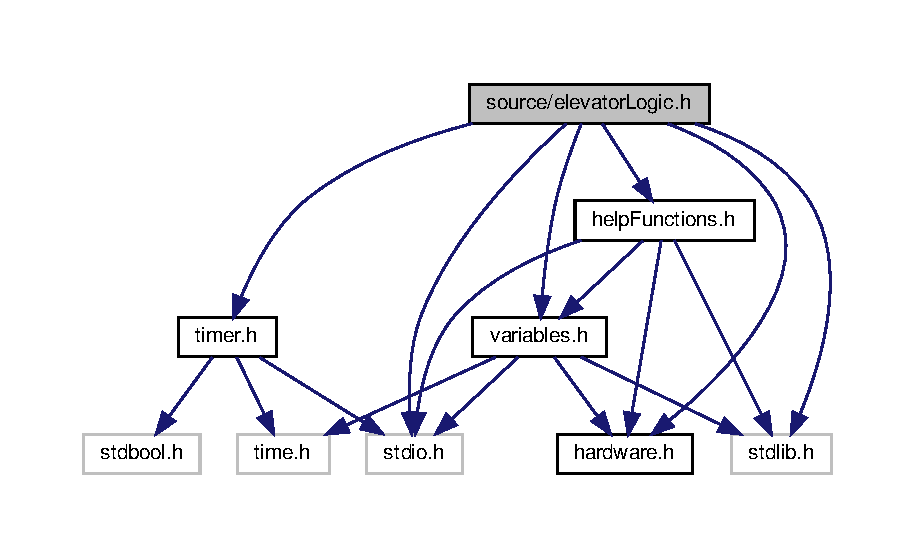
\includegraphics[width=350pt]{elevatorLogic_8h__incl}
\end{center}
\end{figure}
This graph shows which files directly or indirectly include this file\+:
\nopagebreak
\begin{figure}[H]
\begin{center}
\leavevmode
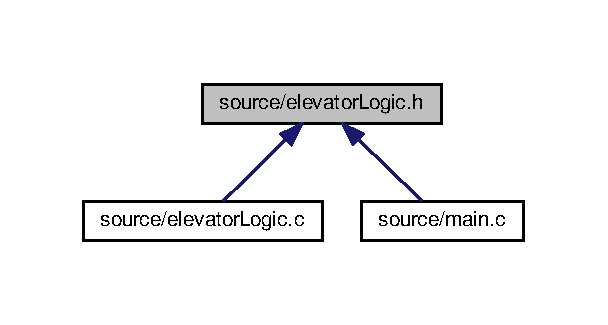
\includegraphics[width=292pt]{elevatorLogic_8h__dep__incl}
\end{center}
\end{figure}
\subsection*{Functions}
\begin{DoxyCompactItemize}
\item 
\mbox{\Hypertarget{elevatorLogic_8h_a5b7e520dd3634bc511e199023a2a4ad5}\label{elevatorLogic_8h_a5b7e520dd3634bc511e199023a2a4ad5}} 
void \hyperlink{elevatorLogic_8h_a5b7e520dd3634bc511e199023a2a4ad5}{initialize\+Elevator} ()
\begin{DoxyCompactList}\small\item\em Resets lights, and drives down until the elevator reaches a floor sensor. Saves this floor as {\ttfamily F\+L\+O\+O\+R.\+current} and {\ttfamily F\+L\+O\+O\+R.\+last}. \end{DoxyCompactList}\item 
int \hyperlink{elevatorLogic_8h_acb58ac12f71a53ca9d454ea0bef0859c}{check\+If\+Stop} ()
\begin{DoxyCompactList}\small\item\em When the elevator is moving and reaches a floor, the floor indicator lights up, {\ttfamily F\+L\+O\+O\+R.\+last} is set, and it decides whether or not to stop at this floor. \end{DoxyCompactList}\item 
\mbox{\Hypertarget{elevatorLogic_8h_a0348ac8c5f50ff4dd510de9905f5d858}\label{elevatorLogic_8h_a0348ac8c5f50ff4dd510de9905f5d858}} 
void \hyperlink{elevatorLogic_8h_a0348ac8c5f50ff4dd510de9905f5d858}{arrive\+Floor} ()
\begin{DoxyCompactList}\small\item\em As long as the {\ttfamily has\+Just\+Left} flag is not set, this function stops the elevator, starts the timer, open the door, and deletes the order to the current floor. \end{DoxyCompactList}\item 
\mbox{\Hypertarget{elevatorLogic_8h_a8259fdde833753b6f23004be29dbb56c}\label{elevatorLogic_8h_a8259fdde833753b6f23004be29dbb56c}} 
void \hyperlink{elevatorLogic_8h_a8259fdde833753b6f23004be29dbb56c}{leave\+Floor} ()
\begin{DoxyCompactList}\small\item\em When the timer reaches 3 seconds and the elevator is not moving, the door is closed and new orders are looked for using {\ttfamily \hyperlink{elevatorLogic_8h_a949e2c521323a4e0d2c37c79c275def5}{update\+Direction()}}. \end{DoxyCompactList}\item 
void \hyperlink{elevatorLogic_8h_a949e2c521323a4e0d2c37c79c275def5}{update\+Direction} ()
\begin{DoxyCompactList}\small\item\em Prioritizes what direction the elevator should go, given {\ttfamily D\+I\+R\+E\+C\+T\+I\+O\+N.\+current}. If the elevator is not moving, {\ttfamily D\+I\+R\+E\+C\+T\+I\+O\+N.\+last} is used to determine which orders to prioritize. \end{DoxyCompactList}\item 
\mbox{\Hypertarget{elevatorLogic_8h_a98ff2b0015e3c6361fdeec413d689f30}\label{elevatorLogic_8h_a98ff2b0015e3c6361fdeec413d689f30}} 
void \hyperlink{elevatorLogic_8h_a98ff2b0015e3c6361fdeec413d689f30}{set\+Orders\+And\+Order\+Lights} ()
\begin{DoxyCompactList}\small\item\em Polls all order buttons, and sets {\ttfamily M\+A\+S\+T\+E\+R\+\_\+\+M\+A\+T\+R\+IX} and the corresponding light if any buttons are pushed. \end{DoxyCompactList}\item 
\mbox{\Hypertarget{elevatorLogic_8h_a19e50b36bc41e271ad3d4e4ac86bb9c3}\label{elevatorLogic_8h_a19e50b36bc41e271ad3d4e4ac86bb9c3}} 
void \hyperlink{elevatorLogic_8h_a19e50b36bc41e271ad3d4e4ac86bb9c3}{stop\+Function} ()
\begin{DoxyCompactList}\small\item\em Stops the elevator, sets {\ttfamily has\+Stopped} to 1 and flushes all orders. If the elevator is at a floor, the door is opened. Sets the stoplight. \end{DoxyCompactList}\item 
\mbox{\Hypertarget{elevatorLogic_8h_af80114ed5f35a4a3facbf60811b46821}\label{elevatorLogic_8h_af80114ed5f35a4a3facbf60811b46821}} 
void \hyperlink{elevatorLogic_8h_af80114ed5f35a4a3facbf60811b46821}{has\+Stopped\+Function} ()
\begin{DoxyCompactList}\small\item\em If the elevator has stopped between two floors, this function determines these two floors and calls {\ttfamily \hyperlink{elevatorLogic_8h_a949e2c521323a4e0d2c37c79c275def5}{update\+Direction()}} with the result as the two parameters. \end{DoxyCompactList}\item 
\mbox{\Hypertarget{elevatorLogic_8h_a629b2358b6d36a8f0312246b38c962eb}\label{elevatorLogic_8h_a629b2358b6d36a8f0312246b38c962eb}} 
void \hyperlink{elevatorLogic_8h_a629b2358b6d36a8f0312246b38c962eb}{check\+For\+Orders\+On\+Current\+Floor} ()
\begin{DoxyCompactList}\small\item\em If the elevator is ordered at its {\ttfamily F\+L\+O\+O\+R.\+current}, {\ttfamily \hyperlink{elevatorLogic_8h_a0348ac8c5f50ff4dd510de9905f5d858}{arrive\+Floor()}} is called. \end{DoxyCompactList}\item 
int \hyperlink{elevatorLogic_8h_a59e7425ac35298bb95a7c2d224a87d98}{check\+For\+Obstruction} ()
\begin{DoxyCompactList}\small\item\em Determines wheter the obstruction switch should have any effect. \end{DoxyCompactList}\end{DoxyCompactItemize}


\subsection{Detailed Description}
Functions that decide what the elevetaor will do at a given time and state. 



\subsection{Function Documentation}
\mbox{\Hypertarget{elevatorLogic_8h_a59e7425ac35298bb95a7c2d224a87d98}\label{elevatorLogic_8h_a59e7425ac35298bb95a7c2d224a87d98}} 
\index{elevator\+Logic.\+h@{elevator\+Logic.\+h}!check\+For\+Obstruction@{check\+For\+Obstruction}}
\index{check\+For\+Obstruction@{check\+For\+Obstruction}!elevator\+Logic.\+h@{elevator\+Logic.\+h}}
\subsubsection{\texorpdfstring{check\+For\+Obstruction()}{checkForObstruction()}}
{\footnotesize\ttfamily int check\+For\+Obstruction (\begin{DoxyParamCaption}{ }\end{DoxyParamCaption})}



Determines wheter the obstruction switch should have any effect. 

\begin{DoxyReturn}{Returns}
1 if the obstruction switch should affect the elevator, 0 if not. 
\end{DoxyReturn}


Definition at line 147 of file elevator\+Logic.\+c.

\mbox{\Hypertarget{elevatorLogic_8h_acb58ac12f71a53ca9d454ea0bef0859c}\label{elevatorLogic_8h_acb58ac12f71a53ca9d454ea0bef0859c}} 
\index{elevator\+Logic.\+h@{elevator\+Logic.\+h}!check\+If\+Stop@{check\+If\+Stop}}
\index{check\+If\+Stop@{check\+If\+Stop}!elevator\+Logic.\+h@{elevator\+Logic.\+h}}
\subsubsection{\texorpdfstring{check\+If\+Stop()}{checkIfStop()}}
{\footnotesize\ttfamily int check\+If\+Stop (\begin{DoxyParamCaption}{ }\end{DoxyParamCaption})}



When the elevator is moving and reaches a floor, the floor indicator lights up, {\ttfamily F\+L\+O\+O\+R.\+last} is set, and it decides whether or not to stop at this floor. 

\begin{DoxyReturn}{Returns}
0 if the elevator is to drive past the floor. 1 to stop. 
\end{DoxyReturn}


Definition at line 25 of file elevator\+Logic.\+c.

\mbox{\Hypertarget{elevatorLogic_8h_a949e2c521323a4e0d2c37c79c275def5}\label{elevatorLogic_8h_a949e2c521323a4e0d2c37c79c275def5}} 
\index{elevator\+Logic.\+h@{elevator\+Logic.\+h}!update\+Direction@{update\+Direction}}
\index{update\+Direction@{update\+Direction}!elevator\+Logic.\+h@{elevator\+Logic.\+h}}
\subsubsection{\texorpdfstring{update\+Direction()}{updateDirection()}}
{\footnotesize\ttfamily void update\+Direction (\begin{DoxyParamCaption}{ }\end{DoxyParamCaption})}



Prioritizes what direction the elevator should go, given {\ttfamily D\+I\+R\+E\+C\+T\+I\+O\+N.\+current}. If the elevator is not moving, {\ttfamily D\+I\+R\+E\+C\+T\+I\+O\+N.\+last} is used to determine which orders to prioritize. 


\begin{DoxyParams}[1]{Parameters}
\mbox{\tt in}  & {\em any\+Orders\+Above} & lets the function know whether the elevator has an order above or not. \\
\hline
\mbox{\tt in}  & {\em any\+Ordersbelow} & lets the function know whether the elevator has an order below or not. \\
\hline
\end{DoxyParams}

\hypertarget{hardware_8h}{}\section{source/hardware.h File Reference}
\label{hardware_8h}\index{source/hardware.\+h@{source/hardware.\+h}}


Driver for the elevator hardware.  


This graph shows which files directly or indirectly include this file\+:
\nopagebreak
\begin{figure}[H]
\begin{center}
\leavevmode
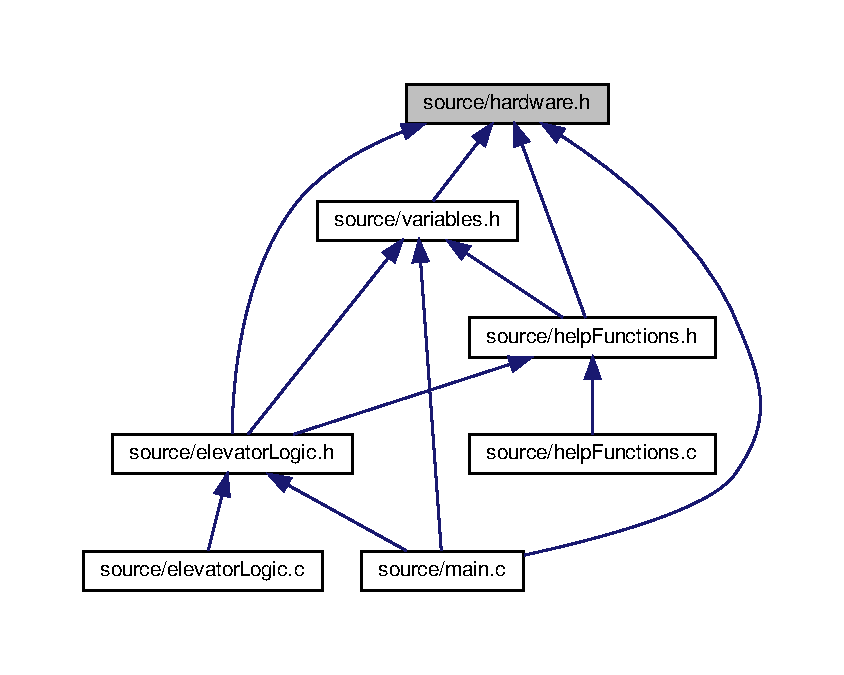
\includegraphics[width=350pt]{hardware_8h__dep__incl}
\end{center}
\end{figure}
\subsection*{Macros}
\begin{DoxyCompactItemize}
\item 
\mbox{\Hypertarget{hardware_8h_ae9e42615eade15633bd8c03b7a271a00}\label{hardware_8h_ae9e42615eade15633bd8c03b7a271a00}} 
\#define {\bfseries H\+A\+R\+D\+W\+A\+R\+E\+\_\+\+N\+U\+M\+B\+E\+R\+\_\+\+O\+F\+\_\+\+F\+L\+O\+O\+RS}~4
\item 
\mbox{\Hypertarget{hardware_8h_ac476fea44244889602251233c8747a83}\label{hardware_8h_ac476fea44244889602251233c8747a83}} 
\#define {\bfseries H\+A\+R\+D\+W\+A\+R\+E\+\_\+\+N\+U\+M\+B\+E\+R\+\_\+\+O\+F\+\_\+\+O\+R\+D\+E\+R\+\_\+\+T\+Y\+P\+ES}~3
\end{DoxyCompactItemize}
\subsection*{Enumerations}
\begin{DoxyCompactItemize}
\item 
\mbox{\Hypertarget{hardware_8h_a2167c399a24df296afc432bcb88228af}\label{hardware_8h_a2167c399a24df296afc432bcb88228af}} 
enum \hyperlink{hardware_8h_a2167c399a24df296afc432bcb88228af}{Hardware\+Movement} \{ {\bfseries H\+A\+R\+D\+W\+A\+R\+E\+\_\+\+M\+O\+V\+E\+M\+E\+N\+T\+\_\+\+UP}, 
{\bfseries H\+A\+R\+D\+W\+A\+R\+E\+\_\+\+M\+O\+V\+E\+M\+E\+N\+T\+\_\+\+D\+O\+WN}, 
{\bfseries H\+A\+R\+D\+W\+A\+R\+E\+\_\+\+M\+O\+V\+E\+M\+E\+N\+T\+\_\+\+S\+T\+OP}
 \}\begin{DoxyCompactList}\small\item\em Movement type used in {\ttfamily hardware\+\_\+command\+\_\+movement}. \end{DoxyCompactList}
\item 
\mbox{\Hypertarget{hardware_8h_a796a8de8ce0ae769d7dbd3327a7bdbe7}\label{hardware_8h_a796a8de8ce0ae769d7dbd3327a7bdbe7}} 
enum \hyperlink{hardware_8h_a796a8de8ce0ae769d7dbd3327a7bdbe7}{Hardware\+Order} \{ {\bfseries H\+A\+R\+D\+W\+A\+R\+E\+\_\+\+O\+R\+D\+E\+R\+\_\+\+UP}, 
{\bfseries H\+A\+R\+D\+W\+A\+R\+E\+\_\+\+O\+R\+D\+E\+R\+\_\+\+D\+O\+WN}, 
{\bfseries H\+A\+R\+D\+W\+A\+R\+E\+\_\+\+O\+R\+D\+E\+R\+\_\+\+I\+N\+S\+I\+DE}
 \}\begin{DoxyCompactList}\small\item\em Order type used in {\ttfamily hardware\+\_\+read\+\_\+order} and in {\ttfamily hardware\+\_\+command\+\_\+order\+\_\+light}. \end{DoxyCompactList}
\end{DoxyCompactItemize}
\subsection*{Functions}
\begin{DoxyCompactItemize}
\item 
int \hyperlink{hardware_8h_a054b8fb8768311d46be58d6a4890d771}{hardware\+\_\+init} ()
\begin{DoxyCompactList}\small\item\em Initializes the elevator control hardware. Must be called once before other calls to the elevator hardware driver. \end{DoxyCompactList}\item 
void \hyperlink{hardware_8h_a01de081ef0510a111053c18cd31afa27}{hardware\+\_\+command\+\_\+movement} (\hyperlink{hardware_8h_a2167c399a24df296afc432bcb88228af}{Hardware\+Movement} movement)
\begin{DoxyCompactList}\small\item\em Commands the elevator to either move up or down, or commands it to halt. \end{DoxyCompactList}\item 
int \hyperlink{hardware_8h_a4a77b27c86675c00b513db3445966804}{hardware\+\_\+read\+\_\+stop\+\_\+signal} ()
\begin{DoxyCompactList}\small\item\em Polls the hardware for the current stop signal. \end{DoxyCompactList}\item 
int \hyperlink{hardware_8h_a459fe57a3ee4bc2a28e8a15b2ab14c2d}{hardware\+\_\+read\+\_\+obstruction\+\_\+signal} ()
\begin{DoxyCompactList}\small\item\em Polls the hardware for the current obstruction signal. \end{DoxyCompactList}\item 
int \hyperlink{hardware_8h_ab048489e6302bb5604aad753f2d7d501}{hardware\+\_\+read\+\_\+floor\+\_\+sensor} (int floor)
\begin{DoxyCompactList}\small\item\em Polls the floor sensor for the given {\ttfamily floor}. \end{DoxyCompactList}\item 
int \hyperlink{hardware_8h_a87917f3aa093fb46ca821a400d011ee8}{hardware\+\_\+read\+\_\+order} (int floor, \hyperlink{hardware_8h_a796a8de8ce0ae769d7dbd3327a7bdbe7}{Hardware\+Order} order\+\_\+type)
\begin{DoxyCompactList}\small\item\em Polls the hardware for the status of orders from floor {\ttfamily floor} of type {\ttfamily order\+\_\+type}. \end{DoxyCompactList}\item 
void \hyperlink{hardware_8h_a80d99ddaa8e7b58c9a88b60ea553c1b6}{hardware\+\_\+command\+\_\+door\+\_\+open} (int door\+\_\+open)
\begin{DoxyCompactList}\small\item\em Commands the hardware to open-\/ or close the elevator door. \end{DoxyCompactList}\item 
void \hyperlink{hardware_8h_a407a6ec035ba357de6aa0fbe55501d1e}{hardware\+\_\+command\+\_\+floor\+\_\+indicator\+\_\+on} (int floor)
\begin{DoxyCompactList}\small\item\em Commands the hardware to turn on the floor indicator for {\ttfamily floor}. All indicators all mutually exclusive; other indicator lights will turn off. \end{DoxyCompactList}\item 
void \hyperlink{hardware_8h_aa75b3ac17f72b25946414f48d0063a10}{hardware\+\_\+command\+\_\+stop\+\_\+light} (int on)
\begin{DoxyCompactList}\small\item\em Sets the light in the panel stop button. \end{DoxyCompactList}\item 
void \hyperlink{hardware_8h_aa9b33faa52f0ec5b614d3e7dc05be140}{hardware\+\_\+command\+\_\+order\+\_\+light} (int floor, \hyperlink{hardware_8h_a796a8de8ce0ae769d7dbd3327a7bdbe7}{Hardware\+Order} order\+\_\+type, int on)
\begin{DoxyCompactList}\small\item\em Sets the light in a button corresponding to an order of type {\ttfamily order\+\_\+type}, at floor {\ttfamily floor}. \end{DoxyCompactList}\item 
int \hyperlink{hardware_8h_a616272b18abac359c7b39497714191f4}{hardware\+\_\+read\+\_\+door\+\_\+open} ()
\begin{DoxyCompactList}\small\item\em Polls the hardware for whether or not the door is open. \end{DoxyCompactList}\end{DoxyCompactItemize}


\subsection{Detailed Description}
Driver for the elevator hardware. 

Neatly wraps up Martin Korsgaard\textquotesingle{}s spaghetti from 2006 ;)

Kolbjørn Austreng 

\subsection{Function Documentation}
\mbox{\Hypertarget{hardware_8h_a80d99ddaa8e7b58c9a88b60ea553c1b6}\label{hardware_8h_a80d99ddaa8e7b58c9a88b60ea553c1b6}} 
\index{hardware.\+h@{hardware.\+h}!hardware\+\_\+command\+\_\+door\+\_\+open@{hardware\+\_\+command\+\_\+door\+\_\+open}}
\index{hardware\+\_\+command\+\_\+door\+\_\+open@{hardware\+\_\+command\+\_\+door\+\_\+open}!hardware.\+h@{hardware.\+h}}
\subsubsection{\texorpdfstring{hardware\+\_\+command\+\_\+door\+\_\+open()}{hardware\_command\_door\_open()}}
{\footnotesize\ttfamily void hardware\+\_\+command\+\_\+door\+\_\+open (\begin{DoxyParamCaption}\item[{int}]{door\+\_\+open }\end{DoxyParamCaption})}



Commands the hardware to open-\/ or close the elevator door. 


\begin{DoxyParams}{Parameters}
{\em door\+\_\+open} & A truthy value (non-\/zero) to open the door; 0 to close. \\
\hline
\end{DoxyParams}
\mbox{\Hypertarget{hardware_8h_a407a6ec035ba357de6aa0fbe55501d1e}\label{hardware_8h_a407a6ec035ba357de6aa0fbe55501d1e}} 
\index{hardware.\+h@{hardware.\+h}!hardware\+\_\+command\+\_\+floor\+\_\+indicator\+\_\+on@{hardware\+\_\+command\+\_\+floor\+\_\+indicator\+\_\+on}}
\index{hardware\+\_\+command\+\_\+floor\+\_\+indicator\+\_\+on@{hardware\+\_\+command\+\_\+floor\+\_\+indicator\+\_\+on}!hardware.\+h@{hardware.\+h}}
\subsubsection{\texorpdfstring{hardware\+\_\+command\+\_\+floor\+\_\+indicator\+\_\+on()}{hardware\_command\_floor\_indicator\_on()}}
{\footnotesize\ttfamily void hardware\+\_\+command\+\_\+floor\+\_\+indicator\+\_\+on (\begin{DoxyParamCaption}\item[{int}]{floor }\end{DoxyParamCaption})}



Commands the hardware to turn on the floor indicator for {\ttfamily floor}. All indicators all mutually exclusive; other indicator lights will turn off. 


\begin{DoxyParams}{Parameters}
{\em floor} & \hyperlink{structFloor}{Floor} to turn on the indicator for.\\
\hline
\end{DoxyParams}
\begin{DoxyWarning}{Warning}
Owing to peculiarities in the hardware construction, there will always be one indicator active. 
\end{DoxyWarning}
\mbox{\Hypertarget{hardware_8h_a01de081ef0510a111053c18cd31afa27}\label{hardware_8h_a01de081ef0510a111053c18cd31afa27}} 
\index{hardware.\+h@{hardware.\+h}!hardware\+\_\+command\+\_\+movement@{hardware\+\_\+command\+\_\+movement}}
\index{hardware\+\_\+command\+\_\+movement@{hardware\+\_\+command\+\_\+movement}!hardware.\+h@{hardware.\+h}}
\subsubsection{\texorpdfstring{hardware\+\_\+command\+\_\+movement()}{hardware\_command\_movement()}}
{\footnotesize\ttfamily void hardware\+\_\+command\+\_\+movement (\begin{DoxyParamCaption}\item[{\hyperlink{hardware_8h_a2167c399a24df296afc432bcb88228af}{Hardware\+Movement}}]{movement }\end{DoxyParamCaption})}



Commands the elevator to either move up or down, or commands it to halt. 


\begin{DoxyParams}{Parameters}
{\em movement} & Commanded movement. \\
\hline
\end{DoxyParams}
\mbox{\Hypertarget{hardware_8h_aa9b33faa52f0ec5b614d3e7dc05be140}\label{hardware_8h_aa9b33faa52f0ec5b614d3e7dc05be140}} 
\index{hardware.\+h@{hardware.\+h}!hardware\+\_\+command\+\_\+order\+\_\+light@{hardware\+\_\+command\+\_\+order\+\_\+light}}
\index{hardware\+\_\+command\+\_\+order\+\_\+light@{hardware\+\_\+command\+\_\+order\+\_\+light}!hardware.\+h@{hardware.\+h}}
\subsubsection{\texorpdfstring{hardware\+\_\+command\+\_\+order\+\_\+light()}{hardware\_command\_order\_light()}}
{\footnotesize\ttfamily void hardware\+\_\+command\+\_\+order\+\_\+light (\begin{DoxyParamCaption}\item[{int}]{floor,  }\item[{\hyperlink{hardware_8h_a796a8de8ce0ae769d7dbd3327a7bdbe7}{Hardware\+Order}}]{order\+\_\+type,  }\item[{int}]{on }\end{DoxyParamCaption})}



Sets the light in a button corresponding to an order of type {\ttfamily order\+\_\+type}, at floor {\ttfamily floor}. 


\begin{DoxyParams}{Parameters}
{\em floor} & The floor of the order indicator. \\
\hline
{\em order\+\_\+type} & The type of order. \\
\hline
{\em on} & A truthy value (non-\/zero) to turn the light on; 0 to turn it off. \\
\hline
\end{DoxyParams}
\mbox{\Hypertarget{hardware_8h_aa75b3ac17f72b25946414f48d0063a10}\label{hardware_8h_aa75b3ac17f72b25946414f48d0063a10}} 
\index{hardware.\+h@{hardware.\+h}!hardware\+\_\+command\+\_\+stop\+\_\+light@{hardware\+\_\+command\+\_\+stop\+\_\+light}}
\index{hardware\+\_\+command\+\_\+stop\+\_\+light@{hardware\+\_\+command\+\_\+stop\+\_\+light}!hardware.\+h@{hardware.\+h}}
\subsubsection{\texorpdfstring{hardware\+\_\+command\+\_\+stop\+\_\+light()}{hardware\_command\_stop\_light()}}
{\footnotesize\ttfamily void hardware\+\_\+command\+\_\+stop\+\_\+light (\begin{DoxyParamCaption}\item[{int}]{on }\end{DoxyParamCaption})}



Sets the light in the panel stop button. 


\begin{DoxyParams}{Parameters}
{\em on} & A truthy value (non-\/zero) to turn the light on; 0 to turn it off. \\
\hline
\end{DoxyParams}
\mbox{\Hypertarget{hardware_8h_a054b8fb8768311d46be58d6a4890d771}\label{hardware_8h_a054b8fb8768311d46be58d6a4890d771}} 
\index{hardware.\+h@{hardware.\+h}!hardware\+\_\+init@{hardware\+\_\+init}}
\index{hardware\+\_\+init@{hardware\+\_\+init}!hardware.\+h@{hardware.\+h}}
\subsubsection{\texorpdfstring{hardware\+\_\+init()}{hardware\_init()}}
{\footnotesize\ttfamily int hardware\+\_\+init (\begin{DoxyParamCaption}{ }\end{DoxyParamCaption})}



Initializes the elevator control hardware. Must be called once before other calls to the elevator hardware driver. 

\begin{DoxyReturn}{Returns}
0 on success. Non-\/zero for failure. 
\end{DoxyReturn}
\mbox{\Hypertarget{hardware_8h_a616272b18abac359c7b39497714191f4}\label{hardware_8h_a616272b18abac359c7b39497714191f4}} 
\index{hardware.\+h@{hardware.\+h}!hardware\+\_\+read\+\_\+door\+\_\+open@{hardware\+\_\+read\+\_\+door\+\_\+open}}
\index{hardware\+\_\+read\+\_\+door\+\_\+open@{hardware\+\_\+read\+\_\+door\+\_\+open}!hardware.\+h@{hardware.\+h}}
\subsubsection{\texorpdfstring{hardware\+\_\+read\+\_\+door\+\_\+open()}{hardware\_read\_door\_open()}}
{\footnotesize\ttfamily int hardware\+\_\+read\+\_\+door\+\_\+open (\begin{DoxyParamCaption}{ }\end{DoxyParamCaption})}



Polls the hardware for whether or not the door is open. 

\begin{DoxyReturn}{Returns}
1 of the door is open, 0 if it is not. 
\end{DoxyReturn}
\mbox{\Hypertarget{hardware_8h_ab048489e6302bb5604aad753f2d7d501}\label{hardware_8h_ab048489e6302bb5604aad753f2d7d501}} 
\index{hardware.\+h@{hardware.\+h}!hardware\+\_\+read\+\_\+floor\+\_\+sensor@{hardware\+\_\+read\+\_\+floor\+\_\+sensor}}
\index{hardware\+\_\+read\+\_\+floor\+\_\+sensor@{hardware\+\_\+read\+\_\+floor\+\_\+sensor}!hardware.\+h@{hardware.\+h}}
\subsubsection{\texorpdfstring{hardware\+\_\+read\+\_\+floor\+\_\+sensor()}{hardware\_read\_floor\_sensor()}}
{\footnotesize\ttfamily int hardware\+\_\+read\+\_\+floor\+\_\+sensor (\begin{DoxyParamCaption}\item[{int}]{floor }\end{DoxyParamCaption})}



Polls the floor sensor for the given {\ttfamily floor}. 


\begin{DoxyParams}{Parameters}
{\em floor} & Inquired floor.\\
\hline
\end{DoxyParams}
\begin{DoxyReturn}{Returns}
1 if the elevator is at {\ttfamily floor}, otherwise 0; 
\end{DoxyReturn}
\mbox{\Hypertarget{hardware_8h_a459fe57a3ee4bc2a28e8a15b2ab14c2d}\label{hardware_8h_a459fe57a3ee4bc2a28e8a15b2ab14c2d}} 
\index{hardware.\+h@{hardware.\+h}!hardware\+\_\+read\+\_\+obstruction\+\_\+signal@{hardware\+\_\+read\+\_\+obstruction\+\_\+signal}}
\index{hardware\+\_\+read\+\_\+obstruction\+\_\+signal@{hardware\+\_\+read\+\_\+obstruction\+\_\+signal}!hardware.\+h@{hardware.\+h}}
\subsubsection{\texorpdfstring{hardware\+\_\+read\+\_\+obstruction\+\_\+signal()}{hardware\_read\_obstruction\_signal()}}
{\footnotesize\ttfamily int hardware\+\_\+read\+\_\+obstruction\+\_\+signal (\begin{DoxyParamCaption}{ }\end{DoxyParamCaption})}



Polls the hardware for the current obstruction signal. 

\begin{DoxyReturn}{Returns}
1 if the obstruction signal is high; 0 if it is low. 
\end{DoxyReturn}
\mbox{\Hypertarget{hardware_8h_a87917f3aa093fb46ca821a400d011ee8}\label{hardware_8h_a87917f3aa093fb46ca821a400d011ee8}} 
\index{hardware.\+h@{hardware.\+h}!hardware\+\_\+read\+\_\+order@{hardware\+\_\+read\+\_\+order}}
\index{hardware\+\_\+read\+\_\+order@{hardware\+\_\+read\+\_\+order}!hardware.\+h@{hardware.\+h}}
\subsubsection{\texorpdfstring{hardware\+\_\+read\+\_\+order()}{hardware\_read\_order()}}
{\footnotesize\ttfamily int hardware\+\_\+read\+\_\+order (\begin{DoxyParamCaption}\item[{int}]{floor,  }\item[{\hyperlink{hardware_8h_a796a8de8ce0ae769d7dbd3327a7bdbe7}{Hardware\+Order}}]{order\+\_\+type }\end{DoxyParamCaption})}



Polls the hardware for the status of orders from floor {\ttfamily floor} of type {\ttfamily order\+\_\+type}. 


\begin{DoxyParams}{Parameters}
{\em floor} & Inquired floor. \\
\hline
{\em order\+\_\+type} & \\
\hline
\end{DoxyParams}
\begin{DoxyReturn}{Returns}
1 if the combination of {\ttfamily floor} and {\ttfamily order\+\_\+type} is being requested, otherwise 0. 
\end{DoxyReturn}
\mbox{\Hypertarget{hardware_8h_a4a77b27c86675c00b513db3445966804}\label{hardware_8h_a4a77b27c86675c00b513db3445966804}} 
\index{hardware.\+h@{hardware.\+h}!hardware\+\_\+read\+\_\+stop\+\_\+signal@{hardware\+\_\+read\+\_\+stop\+\_\+signal}}
\index{hardware\+\_\+read\+\_\+stop\+\_\+signal@{hardware\+\_\+read\+\_\+stop\+\_\+signal}!hardware.\+h@{hardware.\+h}}
\subsubsection{\texorpdfstring{hardware\+\_\+read\+\_\+stop\+\_\+signal()}{hardware\_read\_stop\_signal()}}
{\footnotesize\ttfamily int hardware\+\_\+read\+\_\+stop\+\_\+signal (\begin{DoxyParamCaption}{ }\end{DoxyParamCaption})}



Polls the hardware for the current stop signal. 

\begin{DoxyReturn}{Returns}
1 if the stop signal is high; 0 if it is low. 
\end{DoxyReturn}

\hypertarget{helpFunctions_8c}{}\section{source/help\+Functions.c File Reference}
\label{helpFunctions_8c}\index{source/help\+Functions.\+c@{source/help\+Functions.\+c}}


Implementation file for help\+Functions.  


{\ttfamily \#include \char`\"{}help\+Functions.\+h\char`\"{}}\newline
Include dependency graph for help\+Functions.\+c\+:
\nopagebreak
\begin{figure}[H]
\begin{center}
\leavevmode
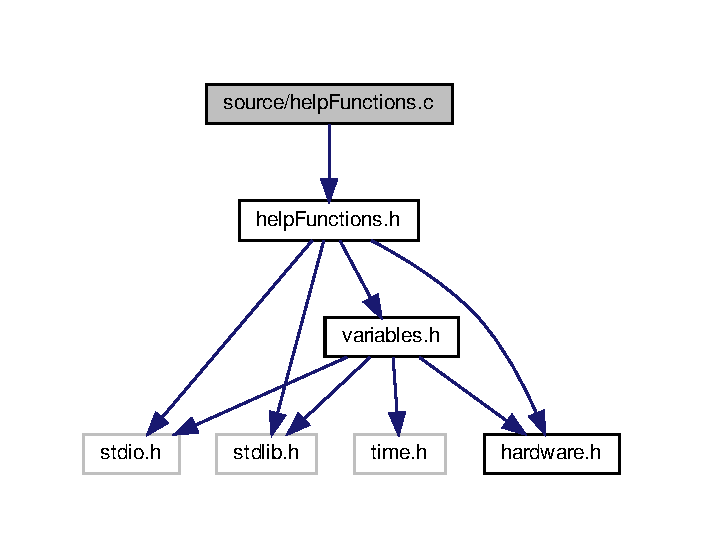
\includegraphics[width=338pt]{helpFunctions_8c__incl}
\end{center}
\end{figure}
\subsection*{Functions}
\begin{DoxyCompactItemize}
\item 
\mbox{\Hypertarget{helpFunctions_8c_a61a48c375e1f6c6081f2ba2d9b2bfa02}\label{helpFunctions_8c_a61a48c375e1f6c6081f2ba2d9b2bfa02}} 
void \hyperlink{helpFunctions_8c_a61a48c375e1f6c6081f2ba2d9b2bfa02}{reset\+Order\+Lights} ()
\begin{DoxyCompactList}\small\item\em Turns of all the order lights in all the floor. \end{DoxyCompactList}\item 
int \hyperlink{helpFunctions_8c_a075e1a379615b6e7f19462d62e7632df}{current\+Floor\+Indicator} ()
\begin{DoxyCompactList}\small\item\em Polls the floor indicator, and investigate whether any floor indicator is active. \end{DoxyCompactList}\item 
int \hyperlink{helpFunctions_8c_a5c77a8069f77f5b3cd9f10825cb42a94}{check\+Orders\+Above} (int temp\+Floor)
\begin{DoxyCompactList}\small\item\em Checks for orders above {\ttfamily temp\+Floor}. \end{DoxyCompactList}\item 
int \hyperlink{helpFunctions_8c_a08aef5b9acc1000125ba037df9407ee6}{check\+Orders\+Below} (int temp\+Floor)
\begin{DoxyCompactList}\small\item\em Checks for orders below {\ttfamily temp\+Floor}. \end{DoxyCompactList}\item 
\mbox{\Hypertarget{helpFunctions_8c_ae2fed0d6439ee5fcf11d14dde925a7f1}\label{helpFunctions_8c_ae2fed0d6439ee5fcf11d14dde925a7f1}} 
void \hyperlink{helpFunctions_8c_ae2fed0d6439ee5fcf11d14dde925a7f1}{delete\+Orders\+And\+Lights\+On\+Current\+Floor} ()
\begin{DoxyCompactList}\small\item\em Turns of all the order lights, and sets every bit in {\ttfamily M\+A\+S\+T\+E\+R\+\_\+\+M\+A\+T\+R\+IX} to 0. \end{DoxyCompactList}\item 
\mbox{\Hypertarget{helpFunctions_8c_a928e32686c7e00c1ecde24c3da3019f7}\label{helpFunctions_8c_a928e32686c7e00c1ecde24c3da3019f7}} 
void \hyperlink{helpFunctions_8c_a928e32686c7e00c1ecde24c3da3019f7}{drive} ()
\begin{DoxyCompactList}\small\item\em Switch on {\ttfamily D\+I\+R\+E\+C\+T\+I\+O\+N.\+current}, drives the elevator. \end{DoxyCompactList}\item 
void \hyperlink{helpFunctions_8c_a8abbfc0f7edd7c8e29b38e188cf353ff}{prioritize\+Above} (int any\+Orders\+Above, int any\+Orders\+Below)
\begin{DoxyCompactList}\small\item\em Sets direction to the elevator based on a case where upwards motion is prefered. \end{DoxyCompactList}\item 
void \hyperlink{helpFunctions_8c_ae891e30f5c407da7548d74526d3dd442}{prioritize\+Below} (int any\+Orders\+Above, int any\+Orders\+Below)
\begin{DoxyCompactList}\small\item\em Sets direction to the elevator based on a case where downwards motion is prefered. \end{DoxyCompactList}\item 
\mbox{\Hypertarget{helpFunctions_8c_a1535383fe7904afaf583005bdf7c8174}\label{helpFunctions_8c_a1535383fe7904afaf583005bdf7c8174}} 
void \hyperlink{helpFunctions_8c_a1535383fe7904afaf583005bdf7c8174}{reset\+Master\+Matrix} ()
\begin{DoxyCompactList}\small\item\em Sets every bit in {\ttfamily M\+A\+S\+T\+E\+R\+\_\+\+M\+A\+T\+R\+IX} to 0. \end{DoxyCompactList}\end{DoxyCompactItemize}


\subsection{Detailed Description}
Implementation file for help\+Functions. 



\subsection{Function Documentation}
\mbox{\Hypertarget{helpFunctions_8c_a5c77a8069f77f5b3cd9f10825cb42a94}\label{helpFunctions_8c_a5c77a8069f77f5b3cd9f10825cb42a94}} 
\index{help\+Functions.\+c@{help\+Functions.\+c}!check\+Orders\+Above@{check\+Orders\+Above}}
\index{check\+Orders\+Above@{check\+Orders\+Above}!help\+Functions.\+c@{help\+Functions.\+c}}
\subsubsection{\texorpdfstring{check\+Orders\+Above()}{checkOrdersAbove()}}
{\footnotesize\ttfamily int check\+Orders\+Above (\begin{DoxyParamCaption}\item[{int}]{temp\+Floor }\end{DoxyParamCaption})}



Checks for orders above {\ttfamily temp\+Floor}. 


\begin{DoxyParams}{Parameters}
{\em temp\+Floor} & the floor number that are used when searching for orders. \\
\hline
\end{DoxyParams}
\begin{DoxyReturn}{Returns}
0 if no orders above . 1 if any orders above . 
\end{DoxyReturn}


Definition at line 25 of file help\+Functions.\+c.

\mbox{\Hypertarget{helpFunctions_8c_a08aef5b9acc1000125ba037df9407ee6}\label{helpFunctions_8c_a08aef5b9acc1000125ba037df9407ee6}} 
\index{help\+Functions.\+c@{help\+Functions.\+c}!check\+Orders\+Below@{check\+Orders\+Below}}
\index{check\+Orders\+Below@{check\+Orders\+Below}!help\+Functions.\+c@{help\+Functions.\+c}}
\subsubsection{\texorpdfstring{check\+Orders\+Below()}{checkOrdersBelow()}}
{\footnotesize\ttfamily int check\+Orders\+Below (\begin{DoxyParamCaption}\item[{int}]{temp\+Floor }\end{DoxyParamCaption})}



Checks for orders below {\ttfamily temp\+Floor}. 


\begin{DoxyParams}{Parameters}
{\em temp\+Floor} & the floor number that are used when searching for orders. \\
\hline
\end{DoxyParams}
\begin{DoxyReturn}{Returns}
0 if no orders below . 1 if any orders below . 
\end{DoxyReturn}


Definition at line 36 of file help\+Functions.\+c.

\mbox{\Hypertarget{helpFunctions_8c_a075e1a379615b6e7f19462d62e7632df}\label{helpFunctions_8c_a075e1a379615b6e7f19462d62e7632df}} 
\index{help\+Functions.\+c@{help\+Functions.\+c}!current\+Floor\+Indicator@{current\+Floor\+Indicator}}
\index{current\+Floor\+Indicator@{current\+Floor\+Indicator}!help\+Functions.\+c@{help\+Functions.\+c}}
\subsubsection{\texorpdfstring{current\+Floor\+Indicator()}{currentFloorIndicator()}}
{\footnotesize\ttfamily int current\+Floor\+Indicator (\begin{DoxyParamCaption}{ }\end{DoxyParamCaption})}



Polls the floor indicator, and investigate whether any floor indicator is active. 

\begin{DoxyReturn}{Returns}
the floor number of the floor indicator that is active. -\/1 if no indicator is active. 
\end{DoxyReturn}


Definition at line 16 of file help\+Functions.\+c.

\mbox{\Hypertarget{helpFunctions_8c_a8abbfc0f7edd7c8e29b38e188cf353ff}\label{helpFunctions_8c_a8abbfc0f7edd7c8e29b38e188cf353ff}} 
\index{help\+Functions.\+c@{help\+Functions.\+c}!prioritize\+Above@{prioritize\+Above}}
\index{prioritize\+Above@{prioritize\+Above}!help\+Functions.\+c@{help\+Functions.\+c}}
\subsubsection{\texorpdfstring{prioritize\+Above()}{prioritizeAbove()}}
{\footnotesize\ttfamily void prioritize\+Above (\begin{DoxyParamCaption}\item[{int}]{any\+Orders\+Above,  }\item[{int}]{any\+Orders\+Below }\end{DoxyParamCaption})}



Sets direction to the elevator based on a case where upwards motion is prefered. 


\begin{DoxyParams}{Parameters}
{\em any\+Orders\+Above} & lets the function know whether the elevator has an order above or not. \\
\hline
{\em any\+Ordersbelow} & lets the function know whether the elevator has an order below or not. {\ttfamily has\+Stopped} this flag gets updated based on the direction the function sets. \\
\hline
\end{DoxyParams}


Definition at line 81 of file help\+Functions.\+c.

\mbox{\Hypertarget{helpFunctions_8c_ae891e30f5c407da7548d74526d3dd442}\label{helpFunctions_8c_ae891e30f5c407da7548d74526d3dd442}} 
\index{help\+Functions.\+c@{help\+Functions.\+c}!prioritize\+Below@{prioritize\+Below}}
\index{prioritize\+Below@{prioritize\+Below}!help\+Functions.\+c@{help\+Functions.\+c}}
\subsubsection{\texorpdfstring{prioritize\+Below()}{prioritizeBelow()}}
{\footnotesize\ttfamily void prioritize\+Below (\begin{DoxyParamCaption}\item[{int}]{any\+Orders\+Above,  }\item[{int}]{any\+Orders\+Below }\end{DoxyParamCaption})}



Sets direction to the elevator based on a case where downwards motion is prefered. 


\begin{DoxyParams}{Parameters}
{\em any\+Orders\+Above} & lets the function know whether the elevator has an order above or not. \\
\hline
{\em any\+Ordersbelow} & lets the function know whether the elevator has an order below or not. {\ttfamily has\+Stopped} this flag gets updated based on the direction the function sets. \\
\hline
\end{DoxyParams}


Definition at line 87 of file help\+Functions.\+c.


\hypertarget{helpFunctions_8h}{}\section{source/help\+Functions.h File Reference}
\label{helpFunctions_8h}\index{source/help\+Functions.\+h@{source/help\+Functions.\+h}}


Small functions with intuitive behavior that are used in {\ttfamily \hyperlink{elevatorLogic_8c}{elevator\+Logic.\+c}}.  


{\ttfamily \#include $<$stdio.\+h$>$}\newline
{\ttfamily \#include $<$stdlib.\+h$>$}\newline
{\ttfamily \#include \char`\"{}variables.\+h\char`\"{}}\newline
{\ttfamily \#include \char`\"{}hardware.\+h\char`\"{}}\newline
Include dependency graph for help\+Functions.\+h\+:
\nopagebreak
\begin{figure}[H]
\begin{center}
\leavevmode
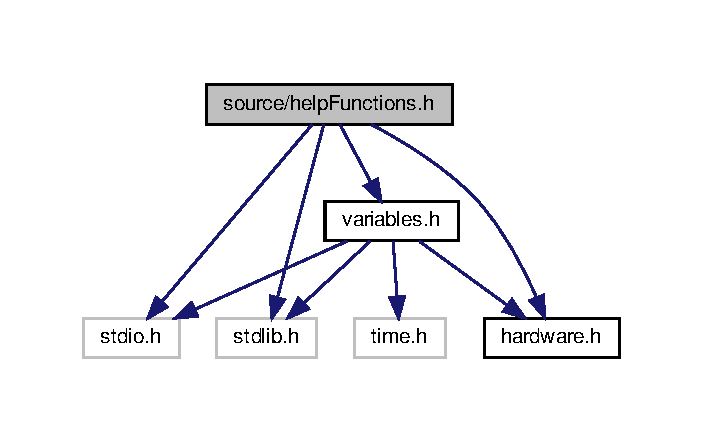
\includegraphics[width=338pt]{helpFunctions_8h__incl}
\end{center}
\end{figure}
This graph shows which files directly or indirectly include this file\+:
\nopagebreak
\begin{figure}[H]
\begin{center}
\leavevmode
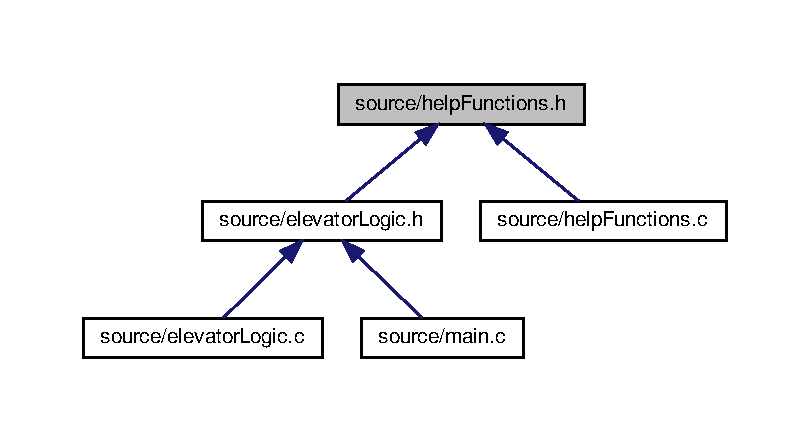
\includegraphics[width=350pt]{helpFunctions_8h__dep__incl}
\end{center}
\end{figure}
\subsection*{Functions}
\begin{DoxyCompactItemize}
\item 
\mbox{\Hypertarget{helpFunctions_8h_a61a48c375e1f6c6081f2ba2d9b2bfa02}\label{helpFunctions_8h_a61a48c375e1f6c6081f2ba2d9b2bfa02}} 
void \hyperlink{helpFunctions_8h_a61a48c375e1f6c6081f2ba2d9b2bfa02}{reset\+Order\+Lights} ()
\begin{DoxyCompactList}\small\item\em Turns of all the order lights in all the floor. \end{DoxyCompactList}\item 
int \hyperlink{helpFunctions_8h_a075e1a379615b6e7f19462d62e7632df}{current\+Floor\+Indicator} ()
\begin{DoxyCompactList}\small\item\em Polls the floor indicator, and investigate whether any floor indicator is active. \end{DoxyCompactList}\item 
int \hyperlink{helpFunctions_8h_a5c77a8069f77f5b3cd9f10825cb42a94}{check\+Orders\+Above} (int temp\+Floor)
\begin{DoxyCompactList}\small\item\em Checks for orders above {\ttfamily temp\+Floor}. \end{DoxyCompactList}\item 
int \hyperlink{helpFunctions_8h_a08aef5b9acc1000125ba037df9407ee6}{check\+Orders\+Below} (int temp\+Floor)
\begin{DoxyCompactList}\small\item\em Checks for orders below {\ttfamily temp\+Floor}. \end{DoxyCompactList}\item 
\mbox{\Hypertarget{helpFunctions_8h_ae2fed0d6439ee5fcf11d14dde925a7f1}\label{helpFunctions_8h_ae2fed0d6439ee5fcf11d14dde925a7f1}} 
void \hyperlink{helpFunctions_8h_ae2fed0d6439ee5fcf11d14dde925a7f1}{delete\+Orders\+And\+Lights\+On\+Current\+Floor} ()
\begin{DoxyCompactList}\small\item\em Turns of all the order lights, and sets every bit in {\ttfamily M\+A\+S\+T\+E\+R\+\_\+\+M\+A\+T\+R\+IX} to 0. \end{DoxyCompactList}\item 
\mbox{\Hypertarget{helpFunctions_8h_a928e32686c7e00c1ecde24c3da3019f7}\label{helpFunctions_8h_a928e32686c7e00c1ecde24c3da3019f7}} 
void \hyperlink{helpFunctions_8h_a928e32686c7e00c1ecde24c3da3019f7}{drive} ()
\begin{DoxyCompactList}\small\item\em Switch on {\ttfamily D\+I\+R\+E\+C\+T\+I\+O\+N.\+current}, drives the elevator. \end{DoxyCompactList}\item 
void \hyperlink{helpFunctions_8h_a8abbfc0f7edd7c8e29b38e188cf353ff}{prioritize\+Above} (int any\+Orders\+Above, int any\+Orders\+Below)
\begin{DoxyCompactList}\small\item\em Sets direction to the elevator based on a case where upwards motion is prefered. \end{DoxyCompactList}\item 
void \hyperlink{helpFunctions_8h_ae891e30f5c407da7548d74526d3dd442}{prioritize\+Below} (int any\+Orders\+Above, int any\+Orders\+Below)
\begin{DoxyCompactList}\small\item\em Sets direction to the elevator based on a case where downwards motion is prefered. \end{DoxyCompactList}\item 
\mbox{\Hypertarget{helpFunctions_8h_a1535383fe7904afaf583005bdf7c8174}\label{helpFunctions_8h_a1535383fe7904afaf583005bdf7c8174}} 
void \hyperlink{helpFunctions_8h_a1535383fe7904afaf583005bdf7c8174}{reset\+Master\+Matrix} ()
\begin{DoxyCompactList}\small\item\em Sets every bit in {\ttfamily M\+A\+S\+T\+E\+R\+\_\+\+M\+A\+T\+R\+IX} to 0. \end{DoxyCompactList}\end{DoxyCompactItemize}


\subsection{Detailed Description}
Small functions with intuitive behavior that are used in {\ttfamily \hyperlink{elevatorLogic_8c}{elevator\+Logic.\+c}}. 



\subsection{Function Documentation}
\mbox{\Hypertarget{helpFunctions_8h_a5c77a8069f77f5b3cd9f10825cb42a94}\label{helpFunctions_8h_a5c77a8069f77f5b3cd9f10825cb42a94}} 
\index{help\+Functions.\+h@{help\+Functions.\+h}!check\+Orders\+Above@{check\+Orders\+Above}}
\index{check\+Orders\+Above@{check\+Orders\+Above}!help\+Functions.\+h@{help\+Functions.\+h}}
\subsubsection{\texorpdfstring{check\+Orders\+Above()}{checkOrdersAbove()}}
{\footnotesize\ttfamily int check\+Orders\+Above (\begin{DoxyParamCaption}\item[{int}]{temp\+Floor }\end{DoxyParamCaption})}



Checks for orders above {\ttfamily temp\+Floor}. 


\begin{DoxyParams}{Parameters}
{\em temp\+Floor} & the floor number that are used when searching for orders. \\
\hline
\end{DoxyParams}
\begin{DoxyReturn}{Returns}
0 if no orders above . 1 if any orders above . 
\end{DoxyReturn}


Definition at line 25 of file help\+Functions.\+c.

\mbox{\Hypertarget{helpFunctions_8h_a08aef5b9acc1000125ba037df9407ee6}\label{helpFunctions_8h_a08aef5b9acc1000125ba037df9407ee6}} 
\index{help\+Functions.\+h@{help\+Functions.\+h}!check\+Orders\+Below@{check\+Orders\+Below}}
\index{check\+Orders\+Below@{check\+Orders\+Below}!help\+Functions.\+h@{help\+Functions.\+h}}
\subsubsection{\texorpdfstring{check\+Orders\+Below()}{checkOrdersBelow()}}
{\footnotesize\ttfamily int check\+Orders\+Below (\begin{DoxyParamCaption}\item[{int}]{temp\+Floor }\end{DoxyParamCaption})}



Checks for orders below {\ttfamily temp\+Floor}. 


\begin{DoxyParams}{Parameters}
{\em temp\+Floor} & the floor number that are used when searching for orders. \\
\hline
\end{DoxyParams}
\begin{DoxyReturn}{Returns}
0 if no orders below . 1 if any orders below . 
\end{DoxyReturn}


Definition at line 36 of file help\+Functions.\+c.

\mbox{\Hypertarget{helpFunctions_8h_a075e1a379615b6e7f19462d62e7632df}\label{helpFunctions_8h_a075e1a379615b6e7f19462d62e7632df}} 
\index{help\+Functions.\+h@{help\+Functions.\+h}!current\+Floor\+Indicator@{current\+Floor\+Indicator}}
\index{current\+Floor\+Indicator@{current\+Floor\+Indicator}!help\+Functions.\+h@{help\+Functions.\+h}}
\subsubsection{\texorpdfstring{current\+Floor\+Indicator()}{currentFloorIndicator()}}
{\footnotesize\ttfamily int current\+Floor\+Indicator (\begin{DoxyParamCaption}{ }\end{DoxyParamCaption})}



Polls the floor indicator, and investigate whether any floor indicator is active. 

\begin{DoxyReturn}{Returns}
the floor number of the floor indicator that is active. -\/1 if no indicator is active. 
\end{DoxyReturn}


Definition at line 16 of file help\+Functions.\+c.

\mbox{\Hypertarget{helpFunctions_8h_a8abbfc0f7edd7c8e29b38e188cf353ff}\label{helpFunctions_8h_a8abbfc0f7edd7c8e29b38e188cf353ff}} 
\index{help\+Functions.\+h@{help\+Functions.\+h}!prioritize\+Above@{prioritize\+Above}}
\index{prioritize\+Above@{prioritize\+Above}!help\+Functions.\+h@{help\+Functions.\+h}}
\subsubsection{\texorpdfstring{prioritize\+Above()}{prioritizeAbove()}}
{\footnotesize\ttfamily void prioritize\+Above (\begin{DoxyParamCaption}\item[{int}]{any\+Orders\+Above,  }\item[{int}]{any\+Orders\+Below }\end{DoxyParamCaption})}



Sets direction to the elevator based on a case where upwards motion is prefered. 


\begin{DoxyParams}{Parameters}
{\em any\+Orders\+Above} & lets the function know whether the elevator has an order above or not. \\
\hline
{\em any\+Ordersbelow} & lets the function know whether the elevator has an order below or not. {\ttfamily has\+Stopped} this flag gets updated based on the direction the function sets. \\
\hline
\end{DoxyParams}


Definition at line 81 of file help\+Functions.\+c.

\mbox{\Hypertarget{helpFunctions_8h_ae891e30f5c407da7548d74526d3dd442}\label{helpFunctions_8h_ae891e30f5c407da7548d74526d3dd442}} 
\index{help\+Functions.\+h@{help\+Functions.\+h}!prioritize\+Below@{prioritize\+Below}}
\index{prioritize\+Below@{prioritize\+Below}!help\+Functions.\+h@{help\+Functions.\+h}}
\subsubsection{\texorpdfstring{prioritize\+Below()}{prioritizeBelow()}}
{\footnotesize\ttfamily void prioritize\+Below (\begin{DoxyParamCaption}\item[{int}]{any\+Orders\+Above,  }\item[{int}]{any\+Orders\+Below }\end{DoxyParamCaption})}



Sets direction to the elevator based on a case where downwards motion is prefered. 


\begin{DoxyParams}{Parameters}
{\em any\+Orders\+Above} & lets the function know whether the elevator has an order above or not. \\
\hline
{\em any\+Ordersbelow} & lets the function know whether the elevator has an order below or not. {\ttfamily has\+Stopped} this flag gets updated based on the direction the function sets. \\
\hline
\end{DoxyParams}


Definition at line 87 of file help\+Functions.\+c.


\hypertarget{main_8c}{}\section{source/main.c File Reference}
\label{main_8c}\index{source/main.\+c@{source/main.\+c}}


The main file of the application.  


{\ttfamily \#include $<$stdio.\+h$>$}\newline
{\ttfamily \#include $<$stdlib.\+h$>$}\newline
{\ttfamily \#include $<$signal.\+h$>$}\newline
{\ttfamily \#include \char`\"{}hardware.\+h\char`\"{}}\newline
{\ttfamily \#include \char`\"{}timer.\+h\char`\"{}}\newline
{\ttfamily \#include \char`\"{}elevator\+Logic.\+h\char`\"{}}\newline
{\ttfamily \#include \char`\"{}variables.\+h\char`\"{}}\newline
Include dependency graph for main.\+c\+:
\nopagebreak
\begin{figure}[H]
\begin{center}
\leavevmode
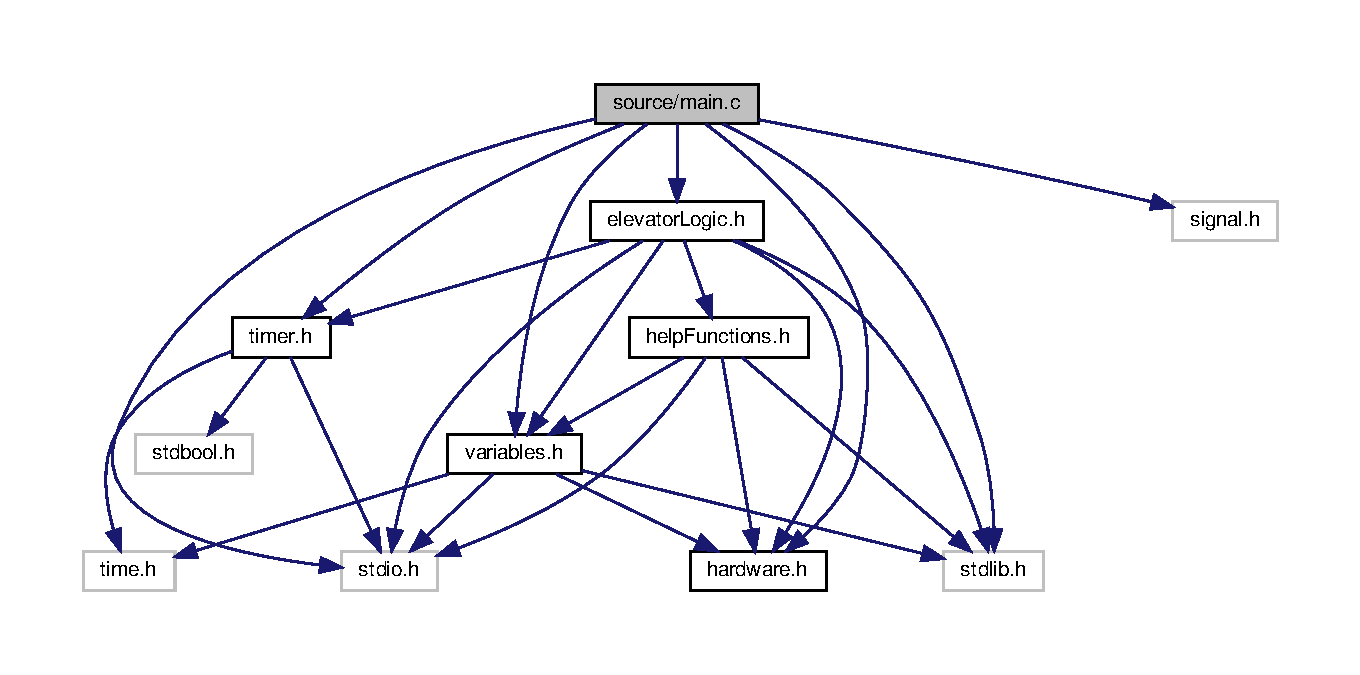
\includegraphics[width=350pt]{main_8c__incl}
\end{center}
\end{figure}
\subsection*{Functions}
\begin{DoxyCompactItemize}
\item 
\mbox{\Hypertarget{main_8c_ae66f6b31b5ad750f1fe042a706a4e3d4}\label{main_8c_ae66f6b31b5ad750f1fe042a706a4e3d4}} 
int {\bfseries main} ()
\end{DoxyCompactItemize}
\subsection*{Variables}
\begin{DoxyCompactItemize}
\item 
\mbox{\Hypertarget{main_8c_a486546968fa5431c0bb5ef280bb3dd8a}\label{main_8c_a486546968fa5431c0bb5ef280bb3dd8a}} 
\hyperlink{structDirection}{Direction} {\bfseries D\+I\+R\+E\+C\+T\+I\+ON} = \{1, 1\}
\item 
\mbox{\Hypertarget{main_8c_a53ea4b6a32d28f4e1bc1f26eb7159ac8}\label{main_8c_a53ea4b6a32d28f4e1bc1f26eb7159ac8}} 
\hyperlink{structFloor}{Floor} {\bfseries F\+L\+O\+OR} = \{0, 0\}
\item 
\mbox{\Hypertarget{main_8c_ae8f980abc1e0175bd1dbf8afab7a8710}\label{main_8c_ae8f980abc1e0175bd1dbf8afab7a8710}} 
int \hyperlink{main_8c_ae8f980abc1e0175bd1dbf8afab7a8710}{M\+A\+S\+T\+E\+R\+\_\+\+M\+A\+T\+R\+IX} \mbox{[}3\mbox{]}\mbox{[}4\mbox{]} = \{\{0, 0, 0, 0\}, \{0, 0, 0, 0\}, \{0, 0, 0, 0\}\}
\begin{DoxyCompactList}\small\item\em A matrix that keeps track of orders. \end{DoxyCompactList}\item 
\mbox{\Hypertarget{main_8c_afe81f8fe13b920b0ee7dd9897afb7f82}\label{main_8c_afe81f8fe13b920b0ee7dd9897afb7f82}} 
time\+\_\+t {\bfseries T\+I\+M\+ER}
\item 
\mbox{\Hypertarget{main_8c_a035d122c383cb498e4694dd187ff33b1}\label{main_8c_a035d122c383cb498e4694dd187ff33b1}} 
int \hyperlink{main_8c_a035d122c383cb498e4694dd187ff33b1}{has\+Stopped} = 0
\begin{DoxyCompactList}\small\item\em A flag thats high when the last order the elevator received was stop. \end{DoxyCompactList}\item 
\mbox{\Hypertarget{main_8c_ab6844c36df1cb99045ec19816f47cb53}\label{main_8c_ab6844c36df1cb99045ec19816f47cb53}} 
int \hyperlink{main_8c_ab6844c36df1cb99045ec19816f47cb53}{has\+Just\+Left} = 0
\begin{DoxyCompactList}\small\item\em A flag that is set high while the elevator has just started moving, but the floor sensor still believes it to be at the floor. \end{DoxyCompactList}\end{DoxyCompactItemize}


\subsection{Detailed Description}
The main file of the application. 


\hypertarget{timer_8c}{}\section{source/timer.c File Reference}
\label{timer_8c}\index{source/timer.\+c@{source/timer.\+c}}


Implementation file for timer.  


{\ttfamily \#include $<$time.\+h$>$}\newline
{\ttfamily \#include \char`\"{}timer.\+h\char`\"{}}\newline
{\ttfamily \#include $<$stdio.\+h$>$}\newline
Include dependency graph for timer.\+c\+:
\nopagebreak
\begin{figure}[H]
\begin{center}
\leavevmode
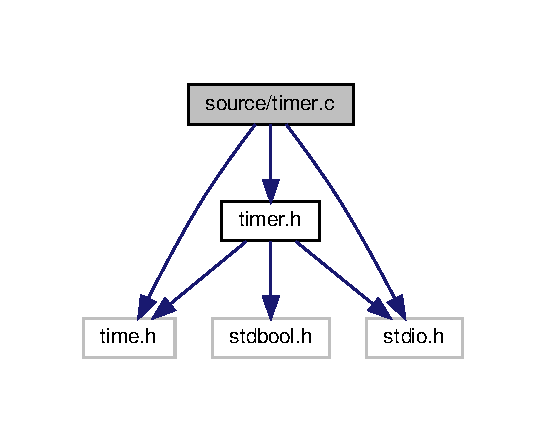
\includegraphics[width=262pt]{timer_8c__incl}
\end{center}
\end{figure}
\subsection*{Functions}
\begin{DoxyCompactItemize}
\item 
void \hyperlink{timer_8c_aec53975ffc59ffaf3080db21af0d2f6e}{start\+Timer} ()
\begin{DoxyCompactList}\small\item\em Starts the timer from scratch. \end{DoxyCompactList}\item 
int \hyperlink{timer_8c_a816c96e6749fe5c521ad07a679ce0135}{timer\+Count} ()
\begin{DoxyCompactList}\small\item\em Returns the time since the last call to  Start\+Timer(). \end{DoxyCompactList}\end{DoxyCompactItemize}
\subsection*{Variables}
\begin{DoxyCompactItemize}
\item 
\mbox{\Hypertarget{timer_8c_afe81f8fe13b920b0ee7dd9897afb7f82}\label{timer_8c_afe81f8fe13b920b0ee7dd9897afb7f82}} 
time\+\_\+t {\bfseries T\+I\+M\+ER}
\end{DoxyCompactItemize}


\subsection{Detailed Description}
Implementation file for timer. 



\subsection{Function Documentation}
\mbox{\Hypertarget{timer_8c_aec53975ffc59ffaf3080db21af0d2f6e}\label{timer_8c_aec53975ffc59ffaf3080db21af0d2f6e}} 
\index{timer.\+c@{timer.\+c}!start\+Timer@{start\+Timer}}
\index{start\+Timer@{start\+Timer}!timer.\+c@{timer.\+c}}
\subsubsection{\texorpdfstring{start\+Timer()}{startTimer()}}
{\footnotesize\ttfamily void start\+Timer (\begin{DoxyParamCaption}{ }\end{DoxyParamCaption})}



Starts the timer from scratch. 


\begin{DoxyParams}[1]{Parameters}
\mbox{\tt out}  & {\em T\+I\+M\+ER} & Global timer variable. \\
\hline
\end{DoxyParams}


Definition at line 12 of file timer.\+c.

\mbox{\Hypertarget{timer_8c_a816c96e6749fe5c521ad07a679ce0135}\label{timer_8c_a816c96e6749fe5c521ad07a679ce0135}} 
\index{timer.\+c@{timer.\+c}!timer\+Count@{timer\+Count}}
\index{timer\+Count@{timer\+Count}!timer.\+c@{timer.\+c}}
\subsubsection{\texorpdfstring{timer\+Count()}{timerCount()}}
{\footnotesize\ttfamily int timer\+Count (\begin{DoxyParamCaption}{ }\end{DoxyParamCaption})}



Returns the time since the last call to  Start\+Timer(). 


\begin{DoxyParams}[1]{Parameters}
\mbox{\tt in}  & {\em T\+I\+M\+ER} & Global timer variable. \\
\hline
\end{DoxyParams}
\begin{DoxyReturn}{Returns}
Returns the number of seconds since the last call to  Start\+Timer(). 
\end{DoxyReturn}


Definition at line 15 of file timer.\+c.


\hypertarget{timer_8h}{}\section{source/timer.h File Reference}
\label{timer_8h}\index{source/timer.\+h@{source/timer.\+h}}


Functions to keep track of how long certain operations has last.  


{\ttfamily \#include $<$stdio.\+h$>$}\newline
{\ttfamily \#include $<$time.\+h$>$}\newline
{\ttfamily \#include $<$stdbool.\+h$>$}\newline
Include dependency graph for timer.\+h\+:
\nopagebreak
\begin{figure}[H]
\begin{center}
\leavevmode
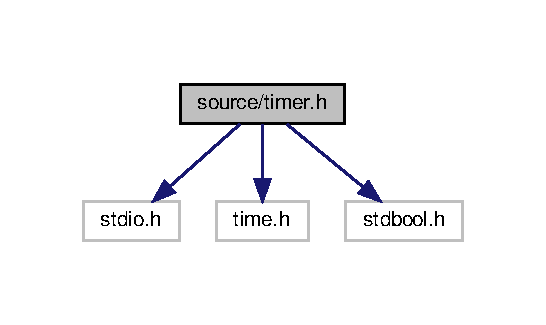
\includegraphics[width=262pt]{timer_8h__incl}
\end{center}
\end{figure}
This graph shows which files directly or indirectly include this file\+:
\nopagebreak
\begin{figure}[H]
\begin{center}
\leavevmode
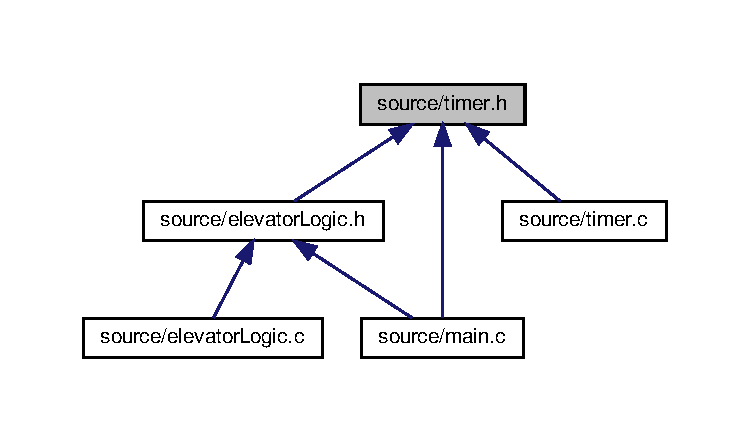
\includegraphics[width=350pt]{timer_8h__dep__incl}
\end{center}
\end{figure}
\subsection*{Macros}
\begin{DoxyCompactItemize}
\item 
\mbox{\Hypertarget{timer_8h_a6e4bae79277e6f8c7c3e5cd1417cfcc4}\label{timer_8h_a6e4bae79277e6f8c7c3e5cd1417cfcc4}} 
\#define {\bfseries T\+I\+M\+E\+R\+\_\+\+W\+A\+I\+T\+\_\+\+C\+O\+N\+S\+T\+A\+NT}~3
\end{DoxyCompactItemize}
\subsection*{Functions}
\begin{DoxyCompactItemize}
\item 
void \hyperlink{timer_8h_aec53975ffc59ffaf3080db21af0d2f6e}{start\+Timer} ()
\begin{DoxyCompactList}\small\item\em Starts the timer from scratch. \end{DoxyCompactList}\item 
int \hyperlink{timer_8h_a816c96e6749fe5c521ad07a679ce0135}{timer\+Count} ()
\begin{DoxyCompactList}\small\item\em Returns the time since the last call to  Start\+Timer(). \end{DoxyCompactList}\end{DoxyCompactItemize}


\subsection{Detailed Description}
Functions to keep track of how long certain operations has last. 



\subsection{Function Documentation}
\mbox{\Hypertarget{timer_8h_aec53975ffc59ffaf3080db21af0d2f6e}\label{timer_8h_aec53975ffc59ffaf3080db21af0d2f6e}} 
\index{timer.\+h@{timer.\+h}!start\+Timer@{start\+Timer}}
\index{start\+Timer@{start\+Timer}!timer.\+h@{timer.\+h}}
\subsubsection{\texorpdfstring{start\+Timer()}{startTimer()}}
{\footnotesize\ttfamily void start\+Timer (\begin{DoxyParamCaption}{ }\end{DoxyParamCaption})}



Starts the timer from scratch. 


\begin{DoxyParams}[1]{Parameters}
\mbox{\tt out}  & {\em T\+I\+M\+ER} & Global timer variable. \\
\hline
\end{DoxyParams}


Definition at line 12 of file timer.\+c.

\mbox{\Hypertarget{timer_8h_a816c96e6749fe5c521ad07a679ce0135}\label{timer_8h_a816c96e6749fe5c521ad07a679ce0135}} 
\index{timer.\+h@{timer.\+h}!timer\+Count@{timer\+Count}}
\index{timer\+Count@{timer\+Count}!timer.\+h@{timer.\+h}}
\subsubsection{\texorpdfstring{timer\+Count()}{timerCount()}}
{\footnotesize\ttfamily int timer\+Count (\begin{DoxyParamCaption}{ }\end{DoxyParamCaption})}



Returns the time since the last call to  Start\+Timer(). 


\begin{DoxyParams}[1]{Parameters}
\mbox{\tt in}  & {\em T\+I\+M\+ER} & Global timer variable. \\
\hline
\end{DoxyParams}
\begin{DoxyReturn}{Returns}
Returns the number of seconds since the last call to  Start\+Timer(). 
\end{DoxyReturn}


Definition at line 15 of file timer.\+c.


\hypertarget{variables_8h}{}\section{source/variables.h File Reference}
\label{variables_8h}\index{source/variables.\+h@{source/variables.\+h}}


Define global variables.  


{\ttfamily \#include $<$stdio.\+h$>$}\newline
{\ttfamily \#include $<$stdlib.\+h$>$}\newline
{\ttfamily \#include $<$time.\+h$>$}\newline
{\ttfamily \#include \char`\"{}hardware.\+h\char`\"{}}\newline
Include dependency graph for variables.\+h\+:
\nopagebreak
\begin{figure}[H]
\begin{center}
\leavevmode
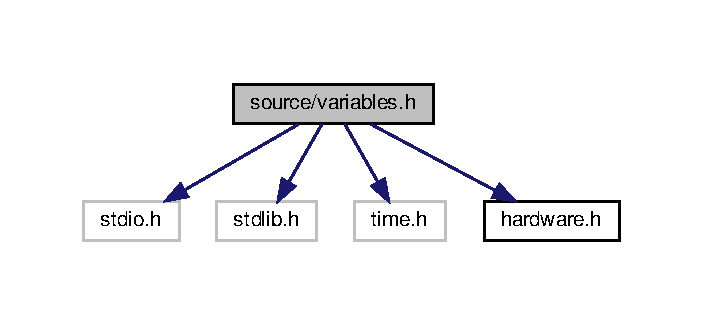
\includegraphics[width=338pt]{variables_8h__incl}
\end{center}
\end{figure}
This graph shows which files directly or indirectly include this file\+:
\nopagebreak
\begin{figure}[H]
\begin{center}
\leavevmode
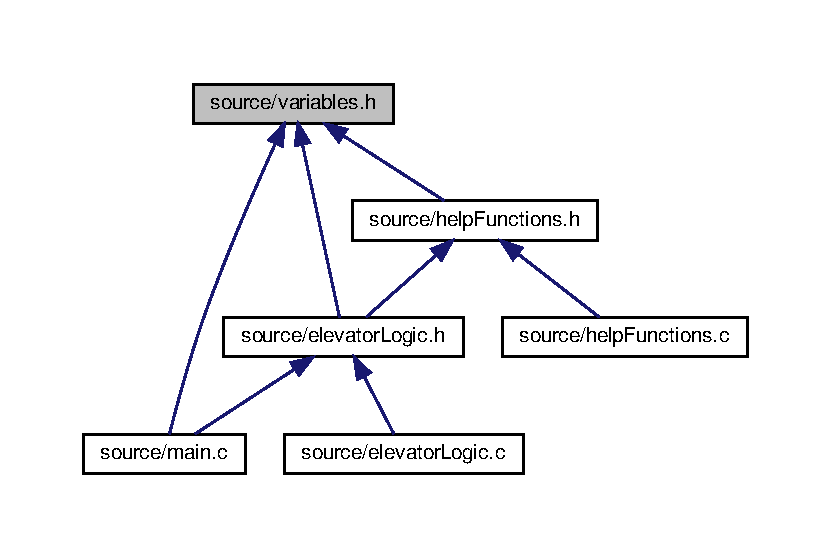
\includegraphics[width=350pt]{variables_8h__dep__incl}
\end{center}
\end{figure}
\subsection*{Data Structures}
\begin{DoxyCompactItemize}
\item 
struct \hyperlink{structFloor}{Floor}
\begin{DoxyCompactList}\small\item\em Define a struct to keep track of current and previous floors. \end{DoxyCompactList}\item 
struct \hyperlink{structDirection}{Direction}
\begin{DoxyCompactList}\small\item\em Define a struct to keep track of current and previous direction. \end{DoxyCompactList}\end{DoxyCompactItemize}
\subsection*{Variables}
\begin{DoxyCompactItemize}
\item 
\mbox{\Hypertarget{variables_8h_a53ea4b6a32d28f4e1bc1f26eb7159ac8}\label{variables_8h_a53ea4b6a32d28f4e1bc1f26eb7159ac8}} 
\hyperlink{structFloor}{Floor} {\bfseries F\+L\+O\+OR}
\item 
\mbox{\Hypertarget{variables_8h_a486546968fa5431c0bb5ef280bb3dd8a}\label{variables_8h_a486546968fa5431c0bb5ef280bb3dd8a}} 
\hyperlink{structDirection}{Direction} {\bfseries D\+I\+R\+E\+C\+T\+I\+ON}
\item 
\mbox{\Hypertarget{variables_8h_ae8f980abc1e0175bd1dbf8afab7a8710}\label{variables_8h_ae8f980abc1e0175bd1dbf8afab7a8710}} 
int \hyperlink{variables_8h_ae8f980abc1e0175bd1dbf8afab7a8710}{M\+A\+S\+T\+E\+R\+\_\+\+M\+A\+T\+R\+IX} \mbox{[}3\mbox{]}\mbox{[}4\mbox{]}
\begin{DoxyCompactList}\small\item\em A matrix that keeps track of orders. \end{DoxyCompactList}\item 
\mbox{\Hypertarget{variables_8h_afe81f8fe13b920b0ee7dd9897afb7f82}\label{variables_8h_afe81f8fe13b920b0ee7dd9897afb7f82}} 
time\+\_\+t {\bfseries T\+I\+M\+ER}
\item 
\mbox{\Hypertarget{variables_8h_a035d122c383cb498e4694dd187ff33b1}\label{variables_8h_a035d122c383cb498e4694dd187ff33b1}} 
int \hyperlink{variables_8h_a035d122c383cb498e4694dd187ff33b1}{has\+Stopped}
\begin{DoxyCompactList}\small\item\em A flag thats high when the last order the elevator received was stop. \end{DoxyCompactList}\item 
\mbox{\Hypertarget{variables_8h_ab6844c36df1cb99045ec19816f47cb53}\label{variables_8h_ab6844c36df1cb99045ec19816f47cb53}} 
int \hyperlink{variables_8h_ab6844c36df1cb99045ec19816f47cb53}{has\+Just\+Left}
\begin{DoxyCompactList}\small\item\em A flag that is set high while the elevator has just started moving, but the floor sensor still believes it to be at the floor. \end{DoxyCompactList}\end{DoxyCompactItemize}


\subsection{Detailed Description}
Define global variables. 


%--- End generated contents ---

% Index
\backmatter
\newpage
\phantomsection
\clearemptydoublepage
\addcontentsline{toc}{chapter}{Index}
\printindex

\end{document}
